%! TEX root=./main.tex

\lecture{3}{Week: 2}{Continue Introduction to C and Integers}

\subsection*{Operators}
Operators and their precedence.

\includegraphics[width=\textwidth]{03_01_operators.png}

\subsubsection{Assignment}
Beside the ternary operator, assignment operators are the only operators which are right-to-left associative while all other operators are left-to-right associative.

As said before, assignments are expressions to (unlike in most other languages).

\subsubsection{Post-/Pre-Increment}
They work as we are used to from Java. We can also apply them to pointers. In that case the pointer value is not incremented by one but by the size of the type of the pointer.

\subsubsection{Casting}
Casting is a prefix operator \code{(newType) value;} which takes a value of a certain type and casts it to another designated type. The bit-representation does usually not change (but sometimes it does). E.g. when casing a small singend integer to a larger singed integer, the leading most significant bits is copied over into the extended region.

\subsection*{Arrays}
An array is a finite vector of values of the same type. They are arranged contiguously in memory. (Most) C compilers do not check array bounds. The indexed as usual, starting at $0$ up to $N-1$ (aka. C++ indexing :P ).

Even though arrays are defined with a certain length, given a array we cannot get its length.

\subsubsection{Basics}
\paragraph{Definition}
The are defined using \code{type name[length];}. E.g. a float array with $5$ elements is defined with \code{float data[5];}.

After the definition, no values are assigned to the array, meaning we do not know what elements the array holds. So we cannot assume that it is all zero or something. In order to initialize each value to zero, we can use \code{type name[length] = \{\};}.

We can also initialize by assigning a set of values like \code{type name[length] = \{val1, val2, ... \}}.

\paragraph{Assignment}
Assignment is done one-by-one using \code{var[i] = val}.

\paragraph{Access}
Arrays are accessed using \code{var[i]}.

\subsubsection{Multidimensional Arrays}
Multidimensional arrays are stored in row-major in a continuous array. Meaning they are stored as $a[0][0], \dots, a[1][0], \dots, a[2][0], \dots, a[2][2]$.

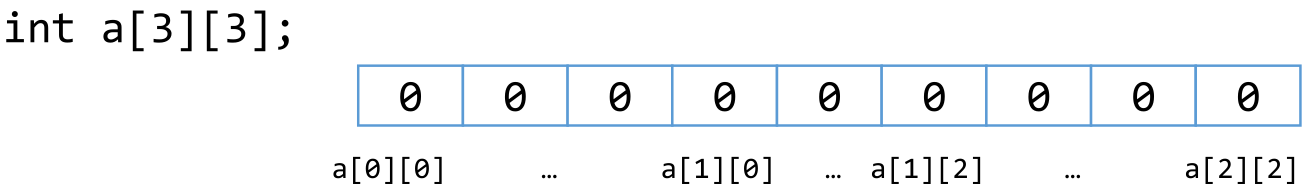
\includegraphics[width=0.8\textwidth]{03_multiDimArray.png}

When viewed as a matrix, the first brackets defines the number of columns and the second bracket the number of rows.

\subsubsection{Strings}
There is no string type in C. Instead strings are an array of chars. The end of the array is marked by the null character \textbackslash 0. We could assign it directly as an array of chars \code{char arr[3] = \{'a', 'b', '\textbackslash 0'\}}. This way we must add the null character explicitly. It is often easier to assign the sting directly as \code{char arr[3]= "ab"}.

Very important is that when setting the length of the array, we keep in mind that the null character requires some space too.

Given that strings have a special termination character, unlike for general arrays, for char arrays we can determine the length of the array given the array.

\paragraph{String Manipulation}
There are no built-in methods for manipulating strings, but there are many libraries which support this. For example \code{<string.h>} is such a library and their manipulation methods have the format \code{strxxx()}.

\code{strcpy} copies a given string, \code{strcat} concatenates two given strings, \code{strcmp} compares two strings of equality etc.

\subsection*{Integers}

\subsubsection{Represent Integers}
Integers are stored as a sequence of bytes. x86 uses little-endian, meaning that the least significant byte comes first.

\subsubsection{Operations}
\paragraph{Bit-Level}
Manipulate single bits of any \textit{integral} data type (long, int, short, char, unsigned). The arguments can be viewed as bit vectors.

\begin{tabular}{c | c}
    $\&$ & and\\
    $|$ & or\\
    $\tilde{}$ & not\\
    $\hat{}$ & xor
\end{tabular}

We can also use the to represent and manipulate sets. We encode bit vectors in a certain way. %something is missing in this sentence

\paragraph{Logical}
Viewing data as true and false where $0$ means false and everything else true. Either of the two states is always returned. They apply to the vector as a whole.

\begin{tabular}{c | c}
    $\&\&$ & and\\
    $||$ & or\\
    $!$ & not
\end{tabular}

\paragraph{Shift}
\begin{itemize}
    \item Left shift: $x << y$ shifts bit-vector $x$ left by $y$ positions
        \begin{itemize}
            \item Fill right with $0$s.
        \end{itemize}
    \item Right shift: $x >> y$ shift bit-vector $x$ right $y$ positions
        \begin{itemize}
            \item Logical shift: fill with $0$s (always applied if int is unsigned)
            \item Arithmetic shift: replicate most significant bit (always applied if int is signed)
        \end{itemize}
\end{itemize}

The behaviour of negative numbers and numbers larger then the vectors is undefined.

\subsubsection{Encoding}
Unsigned integers are encoded in such a way, that with increasing position (LSB to MSB), the factor of two increases: $\sum_{i=0}^{w-1} x_i \cdot 2^i$.

With two's complements encoding we have to consider that the MSB is the sign bit. If is set, $2^{w-1}$ is subtracted of the number represented by the last $w-2$ bits: $-w_{w - 1} \cdot 2^{w - 1} + \sum_{i=0}^{w - 2} x_i \cdot 2^i$.

\subsubsection{Ranges}
\begin{itemize}
    \item UMin $= 0$
    \item UMax $= 2^w -1$
    \item TMin $=-2^{w - 1}$
    \item TMax $=2^{w-1} - 1$
\end{itemize}

Depending on the word size of the number, we can represent different ranges:

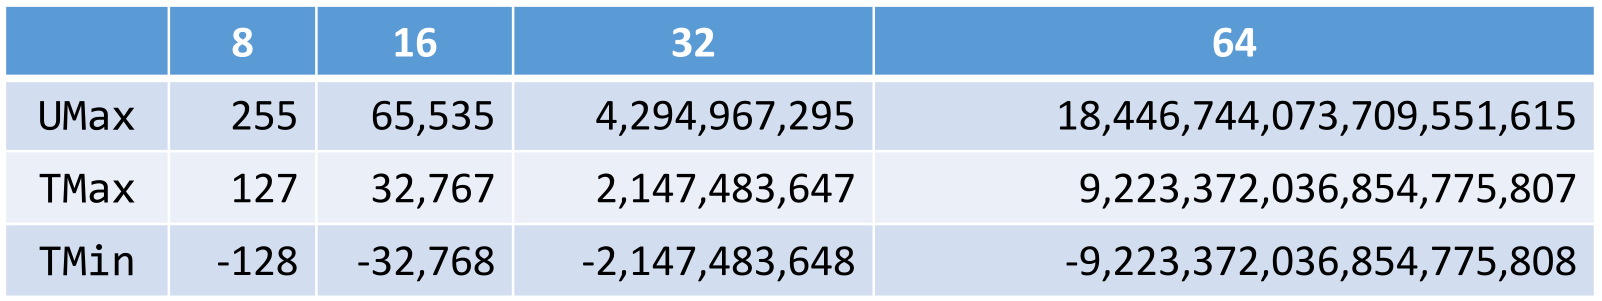
\includegraphics[width=0.8\textwidth]{03_wordSizeRange.png}

From this table we can notice two interesting things:
\begin{enumerate}
    \item $|\text{TMIN}| = |\text{TMAX} + 1$. I.e. we can represent one negative number more than positive (asymmetric range)
    \item UMAX $= 2 \cdot \text{TMAX} + 1$
\end{enumerate}

In practice, we can use \code{<limits.h>} which provides \code{ULONG\_MAX}, \code{LONG\_MAX}, \code{LONG\_MIN}... to get these bounds.

\subsubsection{Visualisation}
When comparing the interpreted signed/unsigned number of a certain bit patters, we see that for the lower halve of numbers, the signed and unsigned numbers are equivalent. Fur the other halve of numbers, i.e. all which have MSB of $1$, we have to add $2^{\text{word size}}$ to get from signed to unsigned. 

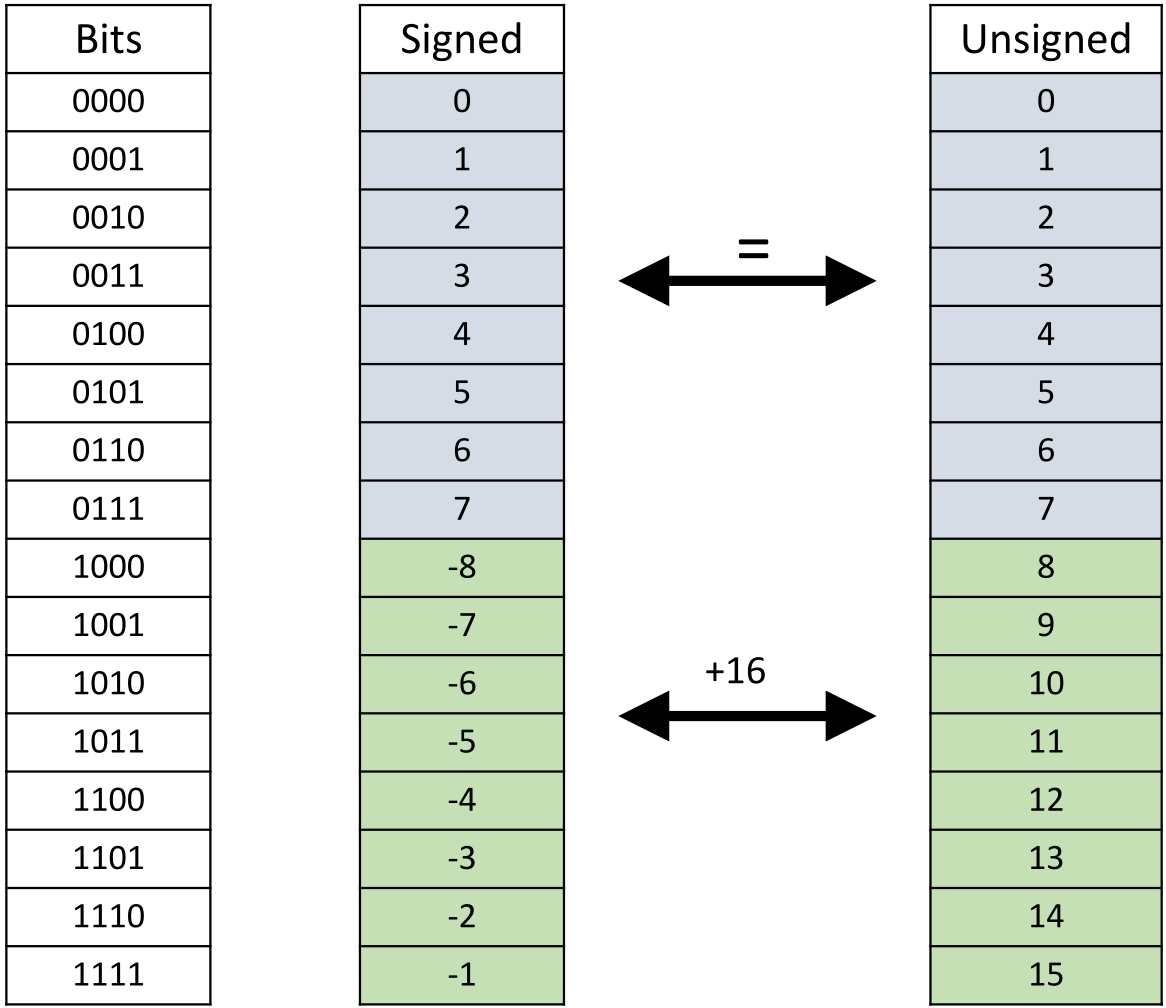
\includegraphics[width=0.8\textwidth]{03_signedUnsignedMap.png}

The difference between signed and unsigned can also be seen as a shift of the ranges.

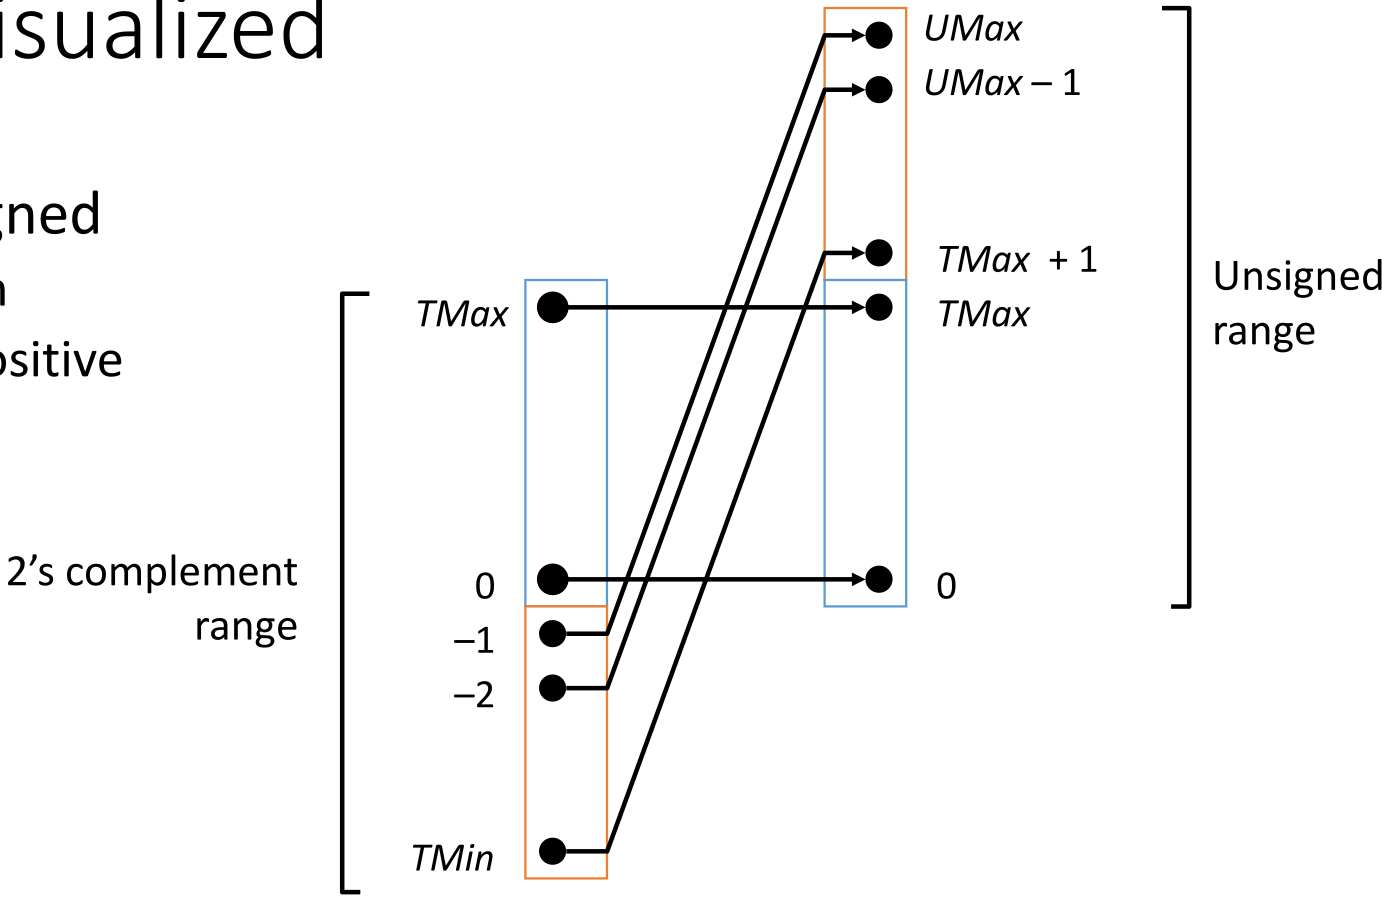
\includegraphics[width=0.8\textwidth]{03_signedUnsignedRange.png}

\subsubsection{Signed vs Unsigned}
By default numbers are considered as signed. In order to get a unsigned number, we have to suffix the number with a \code{U}.

In order to get from one to the other, we have to cast the number. During a cast the bit pattern of the number does not change, it is just interpreted differently.

There are two different ways to cast a number:

\paragraph{Explicit}
Given signed number \code{int a;} we can cast it to unsigned number \code{unsigned b} using \code{b = (unsigned) a;}. The other ways around, casting from unsigned \code{unsigned b} to signed number \code{int a} is done using \code{a = (int) b;}.

\paragraph{Implicit}
This kind of conversion happens when we assign a signed/unsigned number to a unsigned/signed. I.e. given \code{int a; unsigned b;} and we assign \code{a = b;} or \code{b = a;}.

Beside assignments, implicit conversion also happens when we mix signed and unsigned numbers in an expression. It that case the signed number is casted implicitly to a unsigned. 

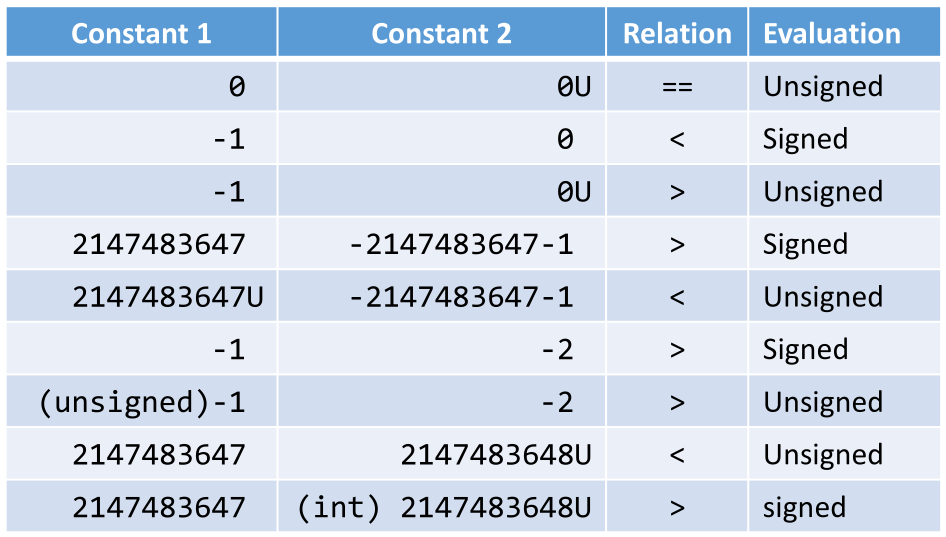
\includegraphics[width=0.8\textwidth]{03_02_numbercasting.png}

If not done by purpose, this can have undesired side effects including security concerns.
